\documentclass[a4paper,onecolumn,10pt]{article}
% Language setting
% Replace `english' with e.g. `spanish' to change the document language
\usepackage[utf8]{inputenc}
\usepackage[spanish]{babel}

% Useful packages
\usepackage{amsmath}
\usepackage{graphicx}
\usepackage{url}

% Title and author info
\title{Taller 1 Big - O }
\author{Camila Andrea Galindo Ruiz - 506222700\\Miguel Daniel Ruiz Silva - 506222719\\Jose David Ramirez Beltran - 506222723}

\begin{document}
\maketitle

\section{Resumen}

\section{Código 1}

\begin{verbatim}
for (int i = 0; i < n; i++) { // O(n)
}
\end{verbatim}

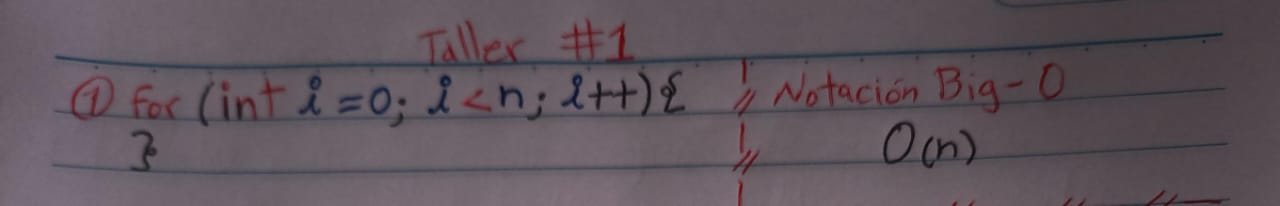
\includegraphics[width=1.15\linewidth]{imagenes/punto 1.jpeg}

\begin{itemize}
    \item La declaración de la variable $i$ y la inicialización de su valor a $0$ tienen una complejidad constante de $O(1)$.
    
    \item La condición del bucle $i < n$ se evalúa $n + 1$ veces, lo que tiene una complejidad de $O(n)$.
    
    \item El incremento de la variable $i$ en cada iteración del bucle también tiene una complejidad de $O(n)$.
    
    \item Por lo que se puede decir que la complejidad total del bucle for es $O(n)$.
    
    \end{itemize}

\section{Código 2}

\begin{verbatim}

for (int i = 0; i < n; i++) { // O(n)
    for (int j = 0; j < m; j++) { // O(m)
    }
}

\end{verbatim}

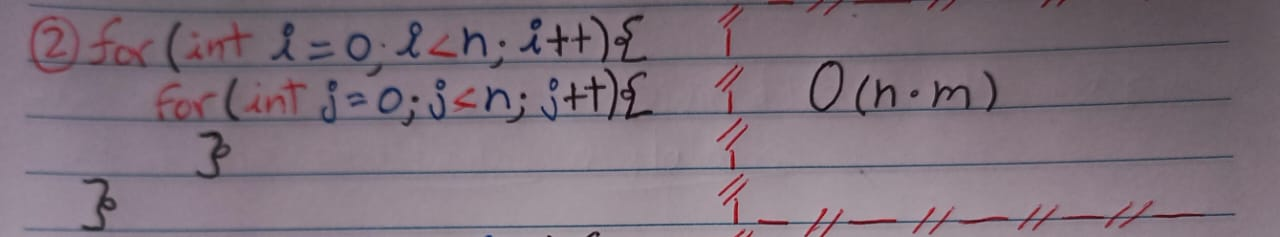
\includegraphics[width=1.15\linewidth]{imagenes/punto 2.jpeg}

\begin{itemize}

    \item La declaración de las variables $i$ y $j$ y la inicialización de sus valores en $0$ tienen una complejidad constante de $O(1)$.
    \item La condición del bucle externo $i < n$ son evaluadas $n + 1$ veces, lo que tiene una complejidad de $O(n)$.
    
    \item La condición del bucle interno $j < m$ se evalúa $m + 1$ veces en cada iteración del bucle externo, lo que tiene una complejidad de $O(m)$.
    
    \item El incremento de las variables $i$ y $j$ en cada iteración de sus bucles también tienen una complejidad de $O(n)$ y $O(m)$.
    \item Por esto la complejidad total del código es $O(n * m)$.

\end{itemize}

\section{Código 3}

\begin{verbatim}

for (int i = 0; i < n; i++) { // O(n)
    for (int j = i; j < n; j++) { // O(n - i)
    }
}

\end{verbatim}

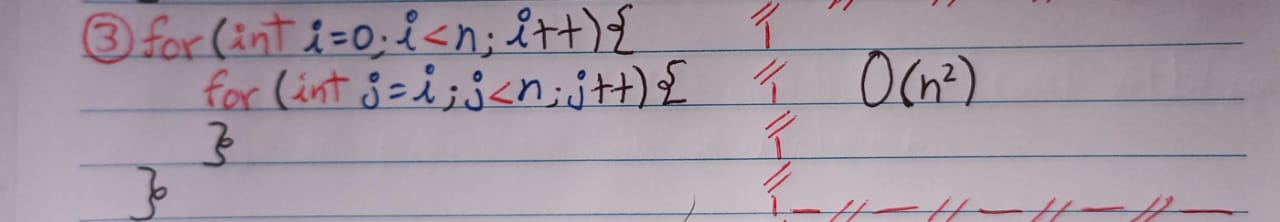
\includegraphics[width=1.15\linewidth]{imagenes/punto 3.jpeg}
\\
\begin{itemize}

    \item La declaración de las variables $i$ y $j$ y la inicialización de sus valores en $0$ e $i$, tienen una complejidad constante de $O(1)$.
    
    \item La condición del bucle externo $i < n$ se evalúa $n + 1$ veces, lo que tiene una complejidad de $O(n)$.
    
    \item La condición del bucle interno $j < n$ se evalúa $n - i + 1$ veces en cada iteración del bucle externo, lo que tiene una complejidad de $O(n - i)$.
    
    \item El incremento de las variables $i$ y $j$ en cada iteración de sus bucles también tienen una complejidad de $O(n)$ y $O(n - i)$.
    
    \item Por esto la complejidad total del código es $O(n^2/2 + n/2) = O(n^2)$.

\end{itemize}

\section{Código 4}

\begin{verbatim}

int index = -1; // O(1)
for (int i = 0; i < n; i++) { // O(n)
    if (array[i] == target) { // O(1)
        index = i; // O(1)
        break; // O(1)
    }
}

\end{verbatim}

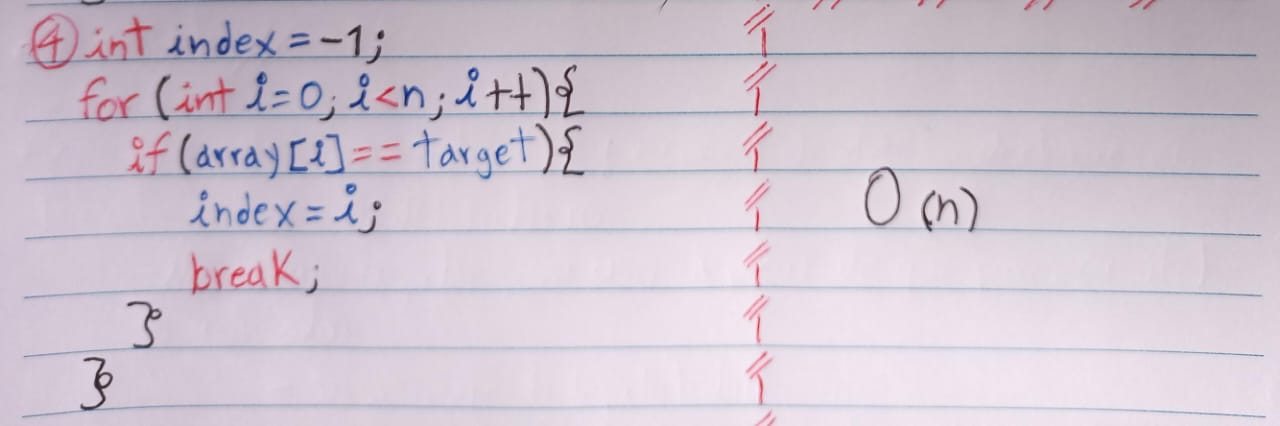
\includegraphics[width=1.15\linewidth]{imagenes/punto 4.jpeg}
\\
\begin{itemize}

    \item La declaración de la variable $index$ y la inicialización de su valor en $-1$ tienen una complejidad constante de $O(1)$.
    
    \item La declaración de la variable $i$ y la inicialización de su valor en $0$ también tienen una complejidad constante de $O(1)$.
    
    \item La condición del bucle $i < n$ se evalúa $n + 1$ veces, lo que tiene una complejidad de $O(n)$.
    
    \item La comparación $array[i] == target$ y la asignación $index = i$ tienen una complejidad constante de $O(1)$.
    
    \item La instrucción break también tiene una complejidad constante de $O(1)$.
    
    \item Por esto la complejidad total del código es $O(n)$.

\end{itemize}

\section{Código 5}

\begin{verbatim}

int left = 0, right = n - 1, index = -1; // O(1)
while (left <= right) { // O(log(n))
    int mid = left + (right - left) / 2; // O(1)
    if (array[mid] == target) { // O(1)
        index = mid; // O(1)
        break; // O(1)
    } else if (array[mid] < target) { // O(1)
        left = mid + 1; // O(1)
    } else {
        right = mid - 1; // O(1)
    }
}

\end{verbatim}

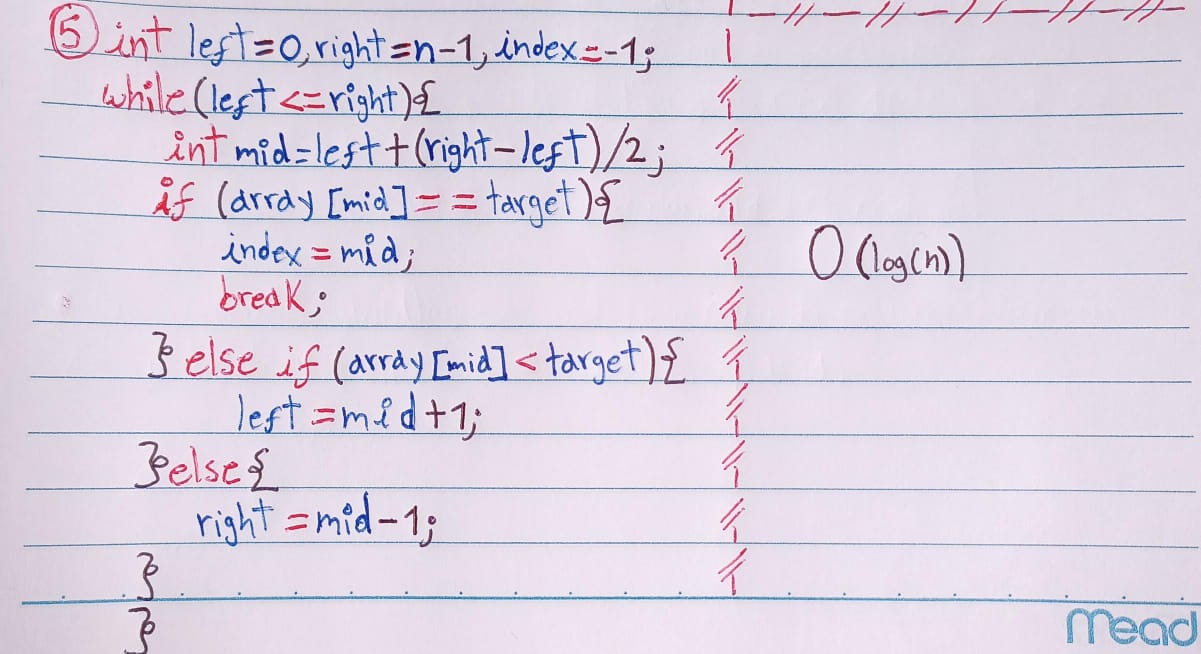
\includegraphics[width=1.15\linewidth]{imagenes/punto 5.jpeg}
\\
\begin{itemize}

    \item La declaración de las variables $left$, $right$ e $index$ y la inicialización de sus valores tienen una complejidad constante de $O(1)$.
    
    \item La condición del bucle while se evalúa hasta que la variable $left$ es mayor que la variable $right$.
    
    \item En cada iteración del bucle el rango de búsqueda se reduce a la mitad, es decir que el número de iteraciónes es proporcional al logaritmo en base 2 del tamaño del rango de búsqueda inicial.
    
    \item Por esto, la complejidad del bucle while es $O(log(n))$, donde $n$ es el tamaño del arreglo $array$.
    
    \item La declaración de la variable $mid$ y la inicialización de su valor tienen una complejidad constante de $O(1)$.
    
    \item Las comparaciónes $array[mid] == target$ y $array[mid] < target$, y también las asignaciónes $index = mid$, $left = mid + 1$ y $right = mid - 1$, también tienen una complejidad constante de $O(1)$.
    
    \item La instrucción break también tiene una complejidad constante de $O(1)$.
    
    \item Por esto la complejidad total del código seria $O(log(n))$.

\end{itemize}

\section{Código 6}

\begin{verbatim}

 int row = 0, col = matrix[0].length - 1, indexRow = -1, indexCol = -1; 
 while (row < matrix.length && col >= 0) {
    if (matrix[row][col] == target) {
        indexRow = row;
        indexCol = col;
        break;
    } else if (matrix[row][col] < target) {
        row++;
    } else {
        col--;
    }
}

\end{verbatim}

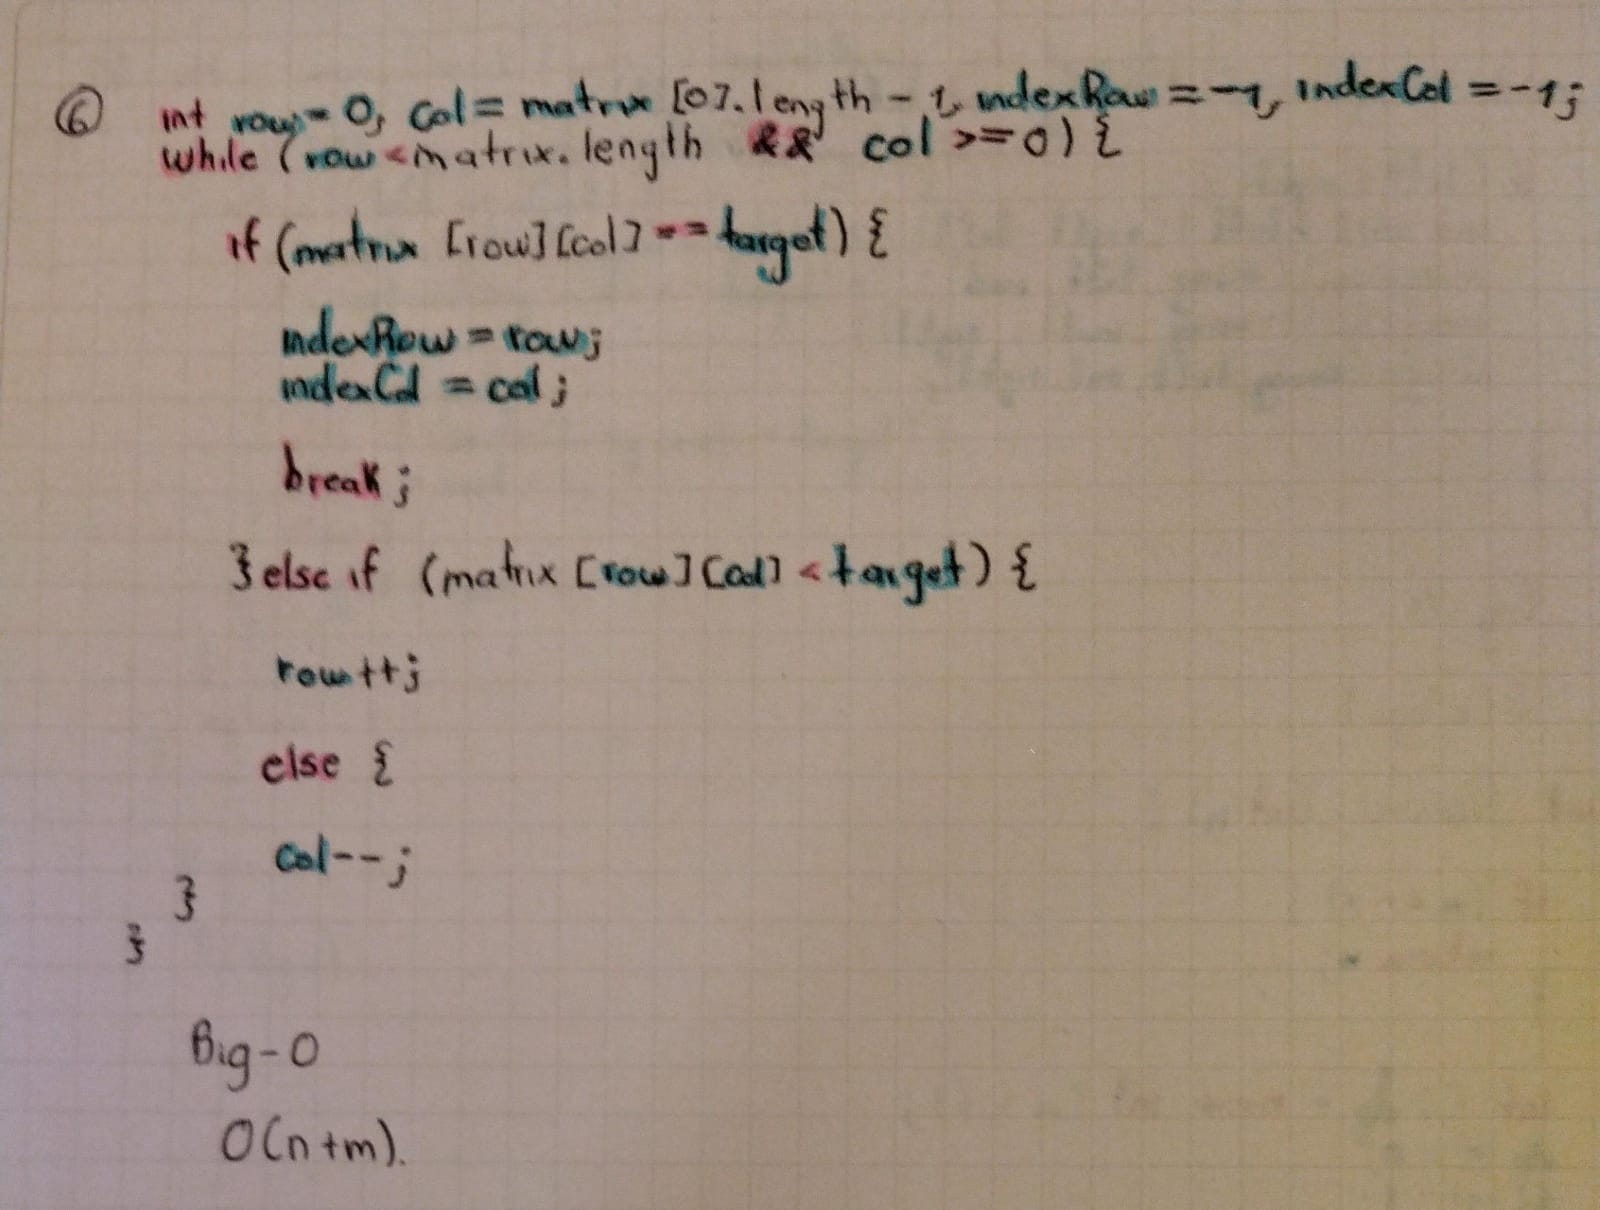
\includegraphics[width=1\linewidth]{imagenes/punto 6.jpeg}
\\

\begin{itemize}

    \item Las líneas \texttt{int row = 0, col = matrix[0].length - 1, indexRow = -1, indexCol = -1;} son asignaciónes y operaciones de tiempo constante: $O(1)$.

    \item El bucle \texttt{while (row < matrix.length \&\& col >= 0)} se ejecuta en función de las dimensiones de la matriz. Supongamos que la matriz tiene "m" filas y "n" columnas. Este bucle se ejecutará en el peor caso hasta que \texttt{row} sea igual a "m" y \texttt{col} sea igual a 0. Por lo tanto, tiene una complejidad de tiempo de $O(m + n)$ en el peor caso.

   \item Dentro del bucle, las comparaciónes \texttt{matrix[row][col] == target} y \texttt{matrix[row][col] < target} son operaciones de tiempo constante: $O(1)$.

   \item Las actualizaciones \texttt{row++} y \texttt{col--} se realizan en cada iteración del bucle y son operaciones de tiempo constante: $O(1)$.

\end{itemize}

\section{Código 7}

\begin{verbatim}

void bubbleSort(int[] array) {
    int n = array.length;
    for (int i = 0; i < n - 1; i++) {
        for (int j = 0; j < n - i - 1; j++) {
            if (array[j] > array[j + 1]) {
                int temp = array[j];
                array[j] = array[j + 1];
                array[j + 1] = temp;
            }
        }
    }
}
 
\end{verbatim}

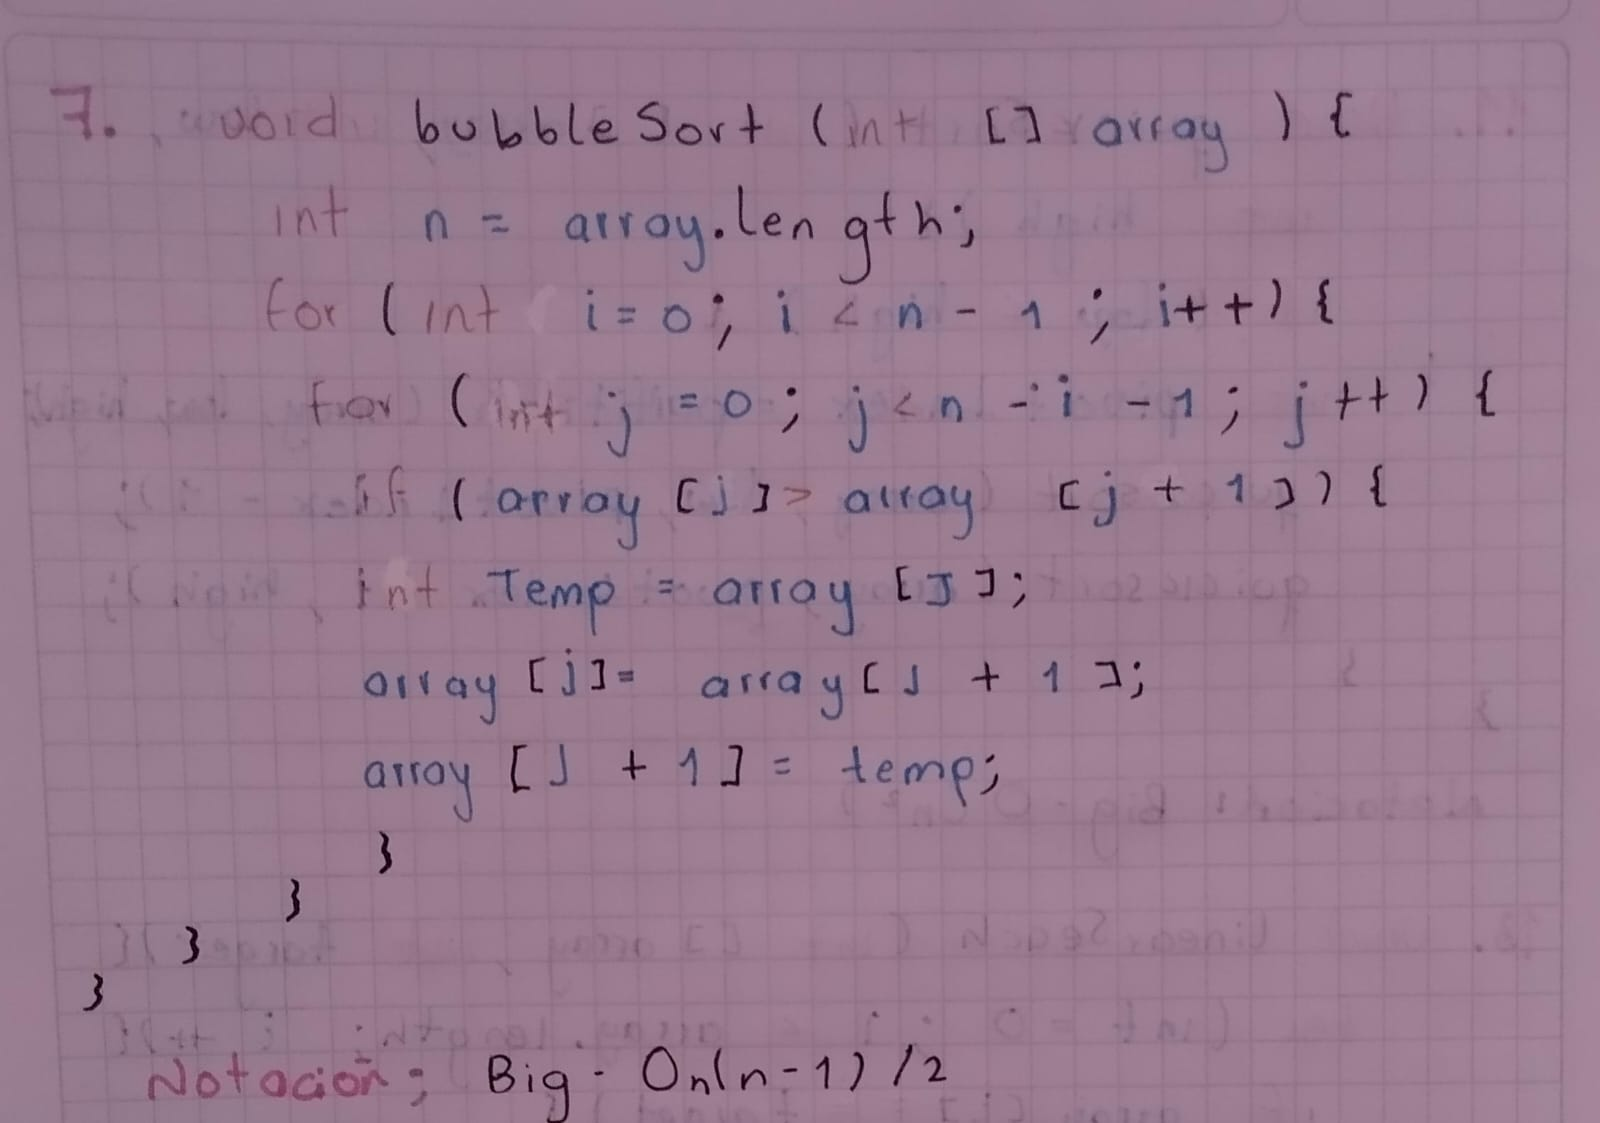
\includegraphics[width=1\linewidth]{imagenes/punto 7.jpeg}
\\
\begin{itemize}

    \item El primero esta en complejidad O (1) porque solo se asigna la longitud del arreglo a una variable.
    
    \item El primer bucle \texttt{for} itera \texttt{n - 1} veces (n es la longitud del arreglo). Por esto su $O(n)$.
   
    \item El segundo bucle \texttt{for} itera \texttt{n - i - 1} veces en cada iteración de \texttt{i}. Hay una comparación y un intercambio que se realizan si se cumple la condicion. En el peor caso, todas estas operaciones se realizan en cada iteración. Lo que nos da una complejidad de $\frac{n(n-1)}{2}$. Esto finalmente se simplifica y nos daria $O(n^2)$
   
    \item En el if las operaciones son constantes por lo que no dependen del arreglo esto hace que su complejidad sea de $O(1)$
    
\end{itemize}

la notacion Big-O: \\

En el peor caso, el arreglo esta completamente desordenado. El bucle externo y el bucle interno se ejecutan completamente, por lo que el numero total de operaciones es $\text(n - 1) * (n - 1)$ lo que nos da un Big - $\text O(n^2)$.
\\

\section{Código 8}

\begin{verbatim}

void selectionSort(int[] array) {
    int n = array.length;
    for (int i = 0; i < n - 1; i++) {
        int minIndex = i;
        for (int j = i + 1; j < n; j++) {
            if (array[j] < array[minIndex]) {
                minIndex = j;
            }
        }
        int temp = array[i];
        array[i] = array[minIndex];
        array[minIndex] = temp;
    }
}

\end{verbatim}

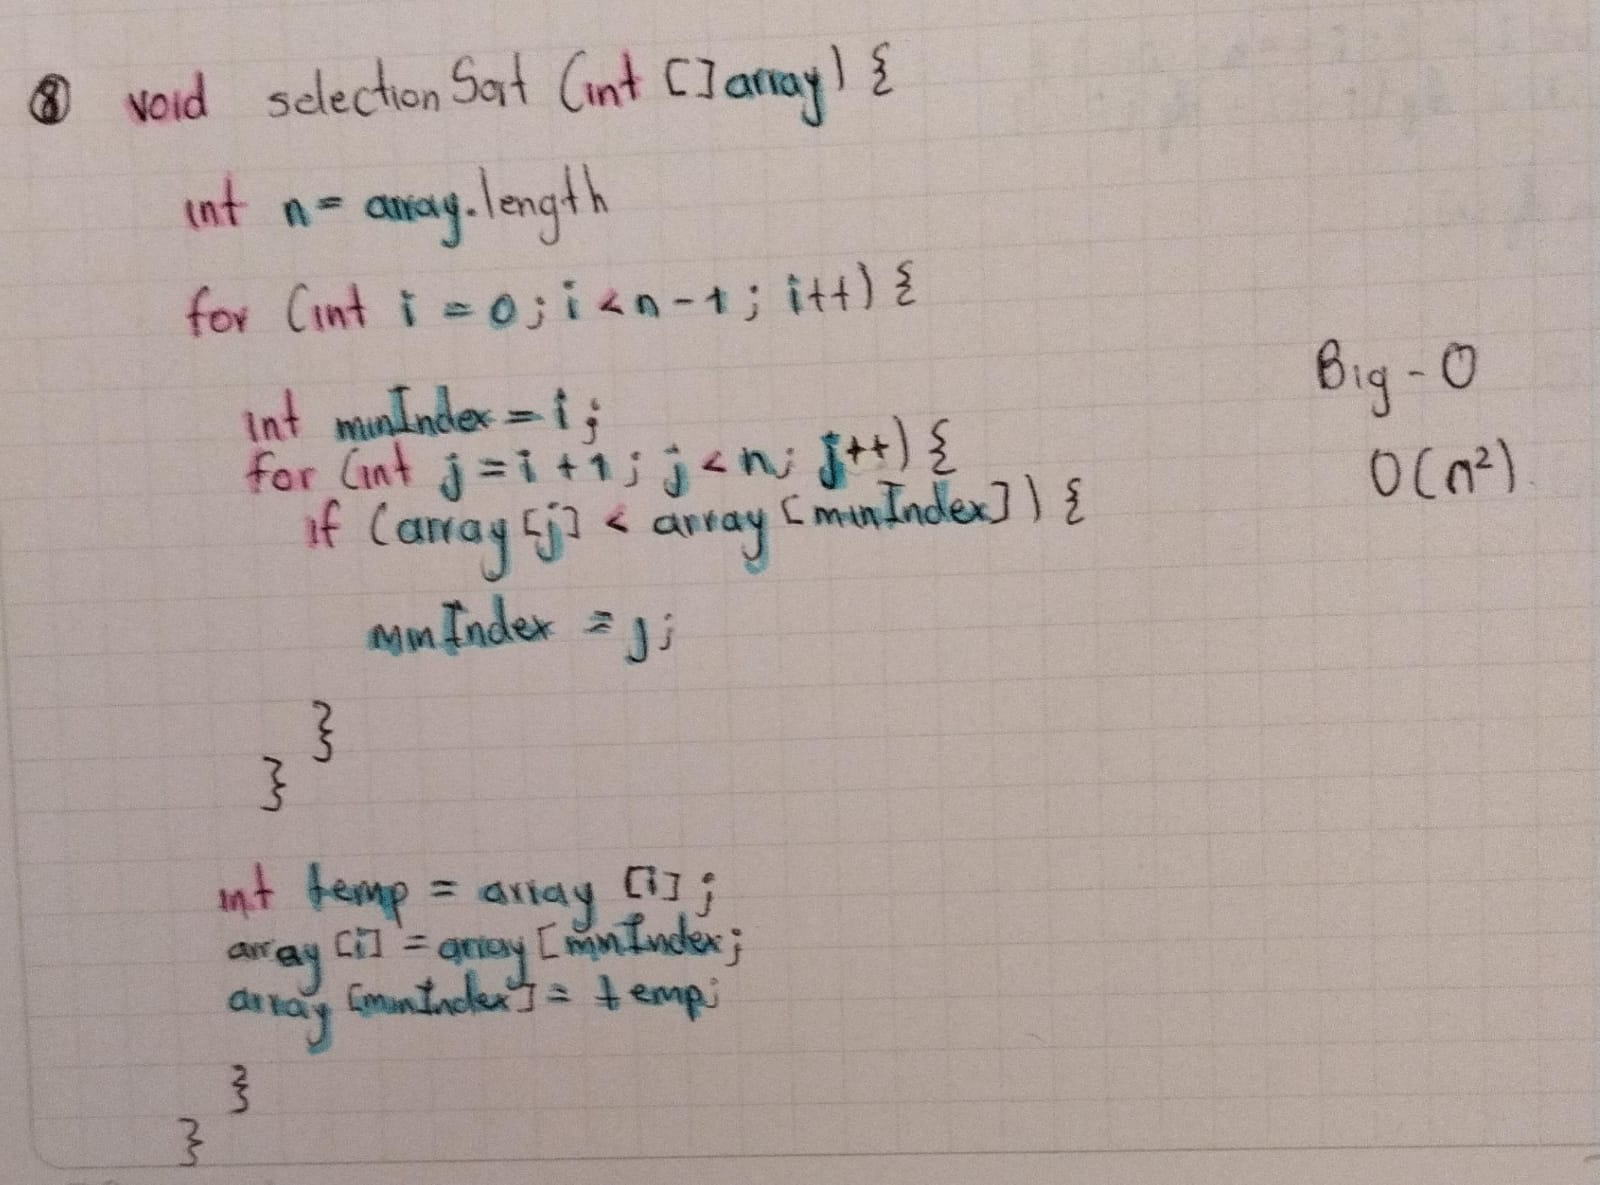
\includegraphics[width=0.95\linewidth]{imagenes/punto 8.jpeg}

\begin{itemize}

    \item La línea \texttt{int n = array.length;} es una asignación y tiene una complejidad de tiempo constante: $O(1)$.

    \item El primer bucle \texttt{for (int i = 0; i < n - 1; i++)} se ejecuta "$n-1$" veces, donde $n$ es el número de elementos en el arreglo. Por lo tanto, tiene una complejidad de tiempo de $O(n)$ en el peor caso.

    \item Dentro del primer bucle, se tiene otro bucle $\texttt{for (int j = i + 1; j < n; j++)}$, que también se ejecuta en función del tamaño del arreglo. Este bucle se ejecuta "$n-i-1$" veces en cada iteración del bucle externo, donde $i$ es el índice del bucle externo. Por lo tanto, la complejidad de este bucle interno es $O(n)$, pero como está anidado dentro del bucle externo, la complejidad total del bucle interno es $O(n^2)$ 

    \item Dentro del bucle interno, hay una comparación  $\texttt{if (array[j] < array[minIndex])}$, que es una operación de tiempo constante: $O(1)$.

    \item Luego, se realiza un intercambio de elementos en el arreglo. Estas operaciones de intercambio también son de tiempo constante: $O(1)$.

\end{itemize}

En resumen, el algoritmo tiene una complejidad de tiempo de $\text O(n^2)$ donde $n$ es el número de elementos en el arreglo.

\section{Código 9}

\begin{verbatim}

void insertionSort(int[] array) {
    int n = array.length;
    for (int i = 1; i < n; i++) {
        int key = array[i];
        int j = i - 1;
        while (j >= 0 && array[j] > key) {
            array[j + 1] = array[j];
            j--;
        }
        array[j + 1] = key;
    }
}

\end{verbatim}

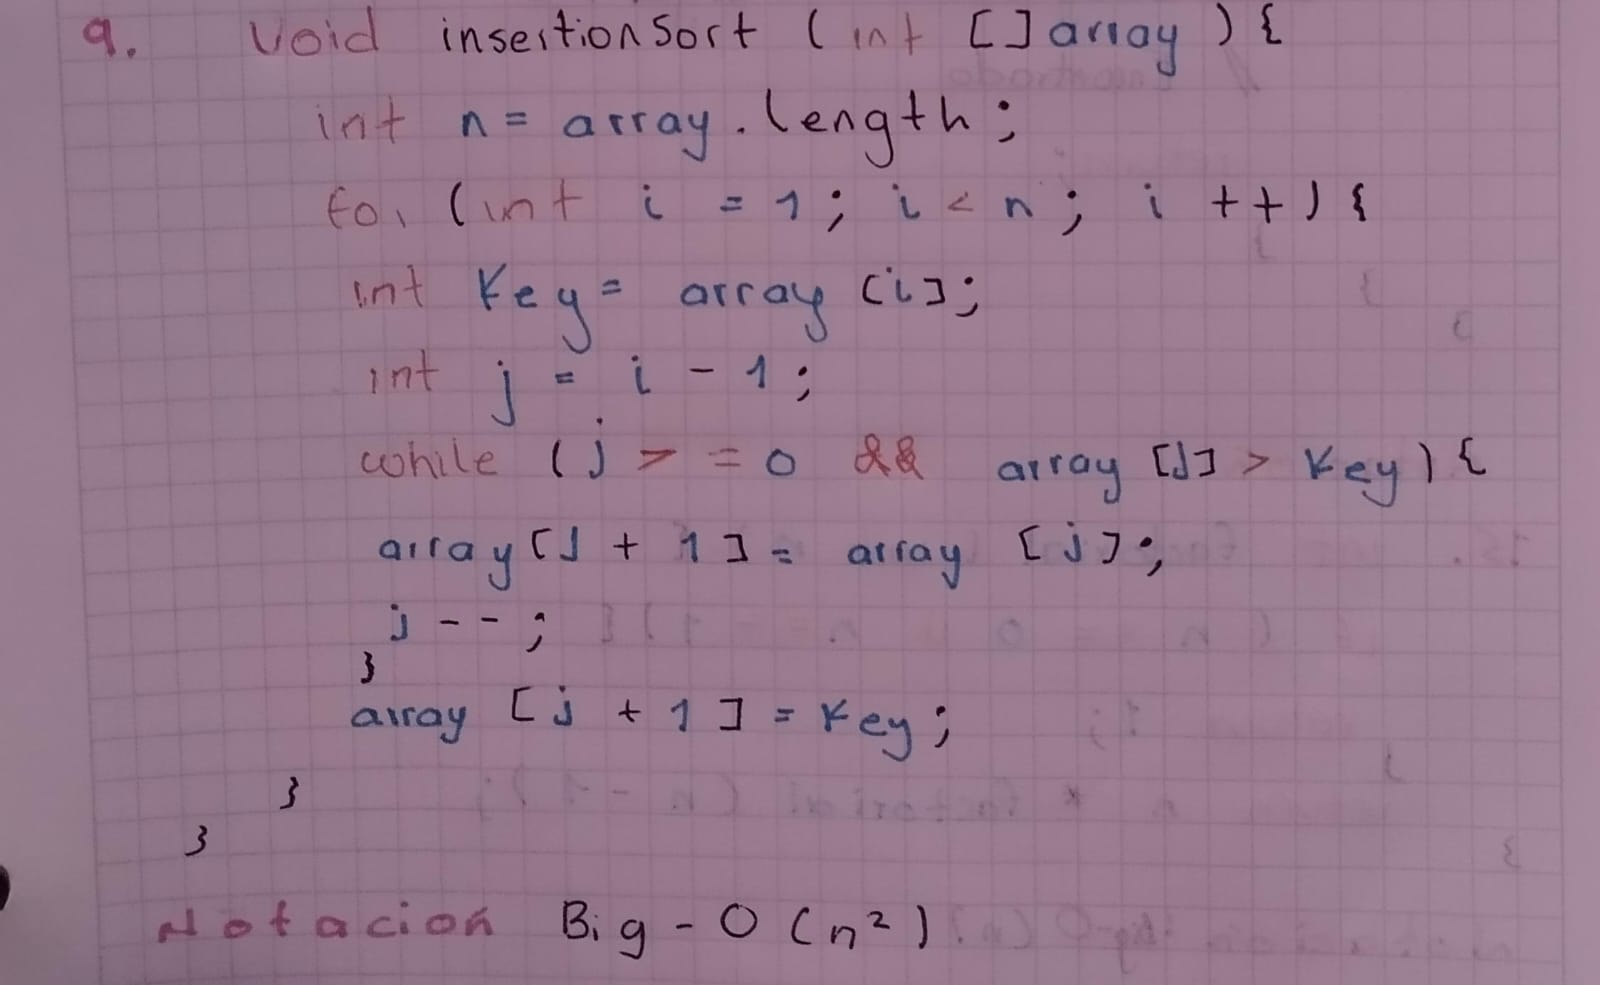
\includegraphics[width=1\linewidth]{imagenes/punto 9.jpeg}
\\ 

\begin{itemize}
    
    \item La complejidad de la segunda linea es de $O(1)$, ya que simplemente asigna el valor de la longitud del arreglo a una variable.
   
    \item El bucle \texttt{for} itera desde $1$ hasta $n – 1$. Por lo tanto, la complejidad de este bucle es $O(n)$.
    
    \item Las operaciones dentro del bucle for son constantes. La asignación \texttt{int key = array[i];} , la asignación \texttt{int j = i - 1;} y la asignación \texttt{array[j + 1] = key;} tienen todas complejidad $O(1)$.\\
   
    \item El bucle \texttt{while} en el peor caso, se ejecuta hasta que $j$ llega a $-1$, lo que significa que realiza un maximo de $i$ iteraciónes. Dado que $i$ puede variar desde $1$ hasta $n - 1$, el bucle \texttt{while} se ejecuta en total $\text 1+\ldots + (n - 1)$ veces, que es proporcional a $\frac{n*(n-1)}{2}$, es decir, $\text O(n^2)$.
    
\end{itemize}

La notación Big-O: \\

La complejidad total del algoritmo en el peor caso es $\text (n^2)$ debido a que el bucle while puede ejecutarse hasta  $\frac{n*(n-1)}{2}$ veces en total.


\section{Código 10}

\begin{verbatim}

    void mergeSort(int[] array, int left, int right) {
    if (left < right) {
        int mid = left + (right - left) / 2;
        mergeSort(array, left, mid);
        mergeSort(array, mid + 1, right);
        merge(array, left, mid, right);
    }
}

\end{verbatim}

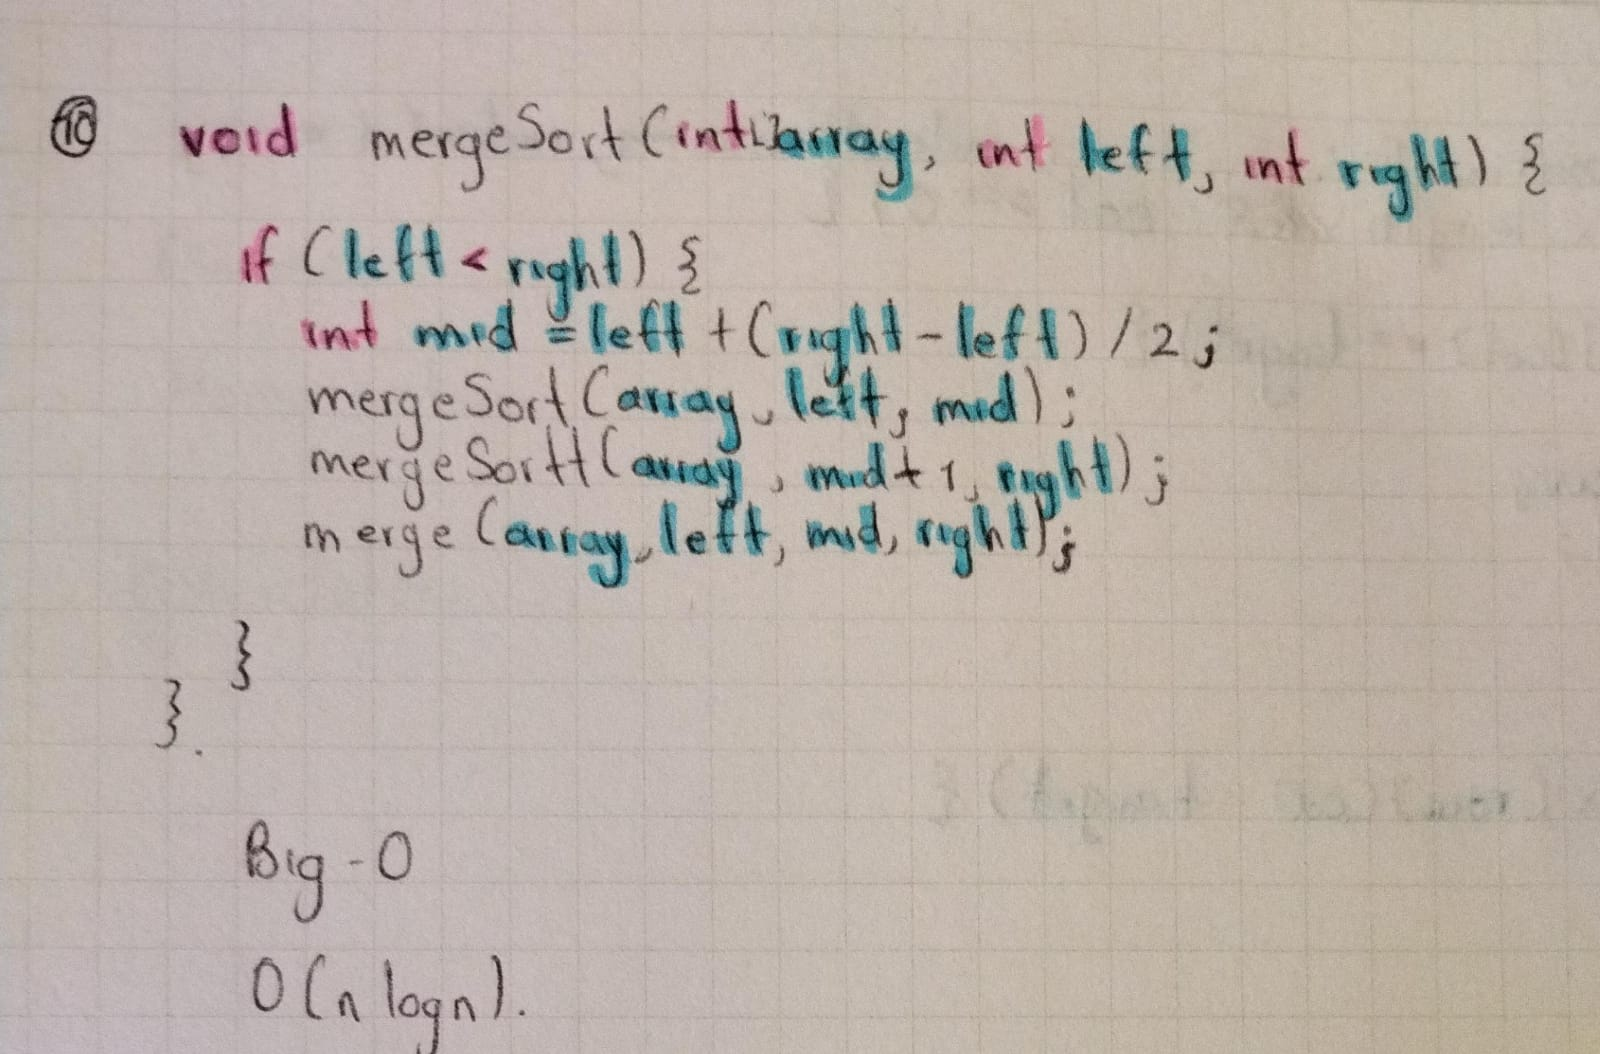
\includegraphics[width=1\linewidth]{imagenes/punto 10.jpeg}

\begin{itemize}
    \item La función mergeSort toma tres argumentos: el arreglo array, el índice izquierdo left, y el índice derecho right. Esta función se llama recursivamente hasta que left sea menor que right. Cuando left es igual o mayor que right, la función se detiene. Por lo tanto, la recursión se realizará hasta que el rango de elementos a ordenar se reduzca a un solo elemento.

    \item En cada llamada recursiva, se calcula el índice medio mid como $\frac{left+(right-left)}{2}$. Esto se hace en tiempo constante: $O(1)$.

    \item Luego, se realiza una llamada recursiva a mergeSort para ordenar la mitad izquierda del arreglo \texttt{(array[left..mid])} y otra llamada para ordenar la mitad derecha \texttt{(array[mid+1..right])}.

    \item Por último la función merge combina las dos mitades ordenadas en una sola matriz. La complejidad de esta función depende de la longitud total de las dos mitades, que es "$\texttt{right - left + 1}$".

    \item El tiempo que lleva combinar dos mitades de longitud $n$ es $O(n)$, y dado que el algoritmo se divide en mitades logarítmicamente (se ejecuta $\text log_2(n)$ veces), la complejidad total del merge sort es $\text O(n log n)$.

\end{itemize}

\section{Código 11}

\begin{verbatim}

void quickSort(int[] array, int low, int high) {
if (low < high) { // O(1)
        int pivotIndex = partition(array, low, high); // O(n)
        quickSort(array, low, pivotIndex - 1); // Recursion
        quickSort(array, pivotIndex + 1, high); // Recursion  
   }
}

\end{verbatim}

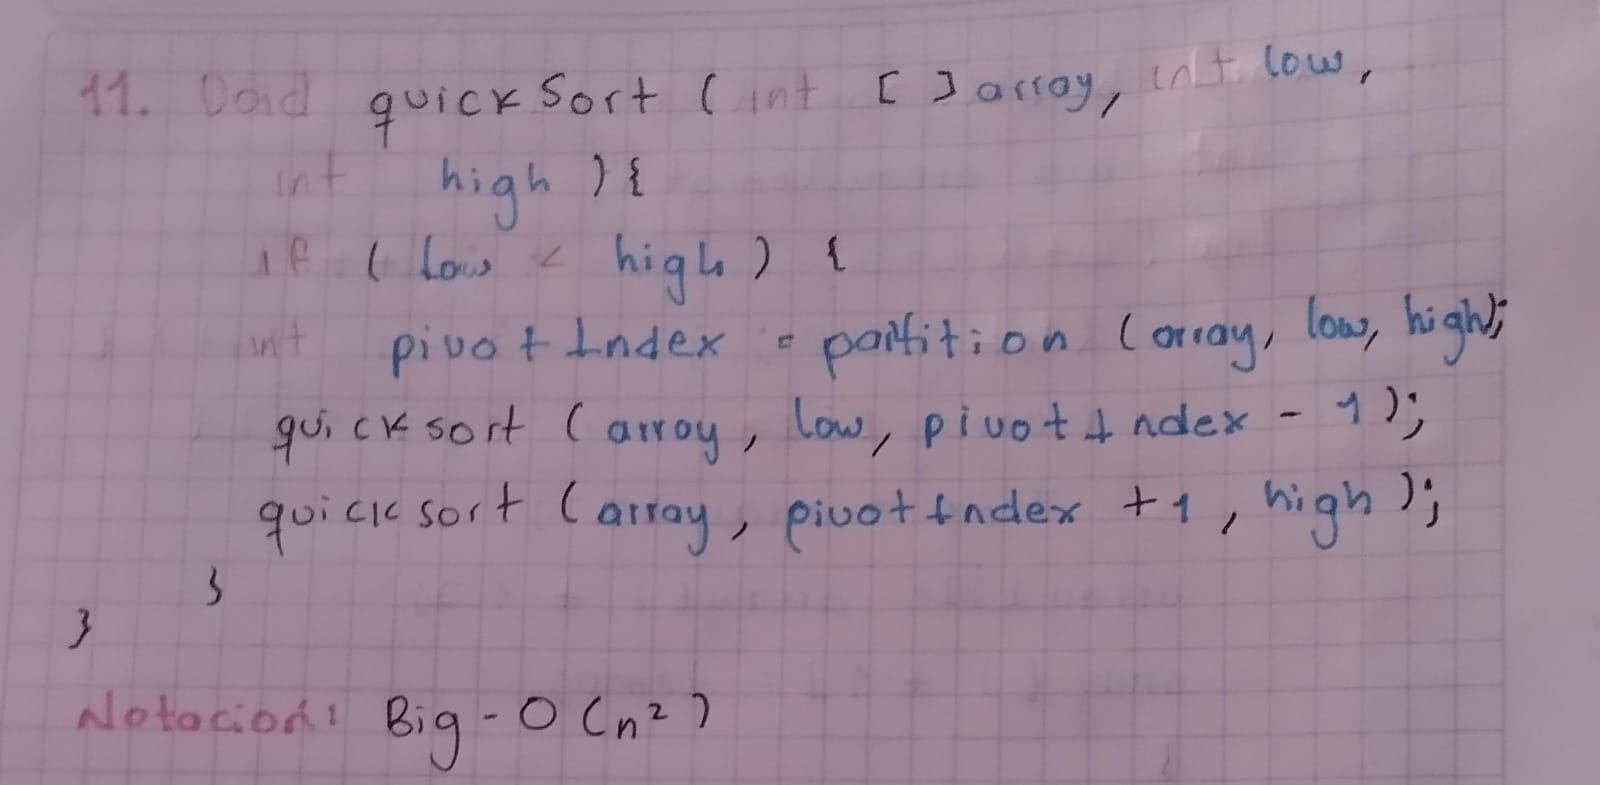
\includegraphics[width=1\linewidth]{imagenes/punto 11.jpeg}

\begin{itemize}

    \item La linea del \texttt{if} verifica si low es menor que high. Esto tiene una complejidad constante $O(1)$.
    
    \item La linea 3 llama a una funcion partition de QuickSort que tiene una complejidad de $O(n)$, ya que implica recorrer el arreglo para dividirlo en dos subarreglos. 
    
    \item Las siguientes dos lineas son llamadas recursivas a quickSort para los dos subarreglos generados por la partición. En el mejor caso, el arreglo se divide en mitades iguales en cada nivel, lo que lleva a una profundidad del arbol de recursion de  $\text log_2(n)$. Por lo tanto, la cantidad de trabajo en cada nivel se multiplica por la cantidad de niveles, dando como resultado una complejidad de  $\text O(n log n)$.
    
\end{itemize}

Notacion Big- O:\\
La complejidad del algoritmo es en el peor caso, donde la partición siempre genera un subarreglo de tamaño 0 y otro de tamaño $n-1$, la complejidad sería $\text O(n^2),$ lo que puede suceder si la elección del pivote es siempre el elemento más pequeño o más grande en un arreglo ya ordenado.

\section{Código 12}

\begin{verbatim}
    
    int fibonacci(int n) {
    if (n <= 1) {
        return n;
    }
    int[] dp = new int[n + 1];
    dp[0] = 0;
    dp[1] = 1;
    for (int i = 2; i <= n; i++) {
        dp[i] = dp[i - 1] + dp[i - 2];
    }
    return dp[n];
}

\end{verbatim}

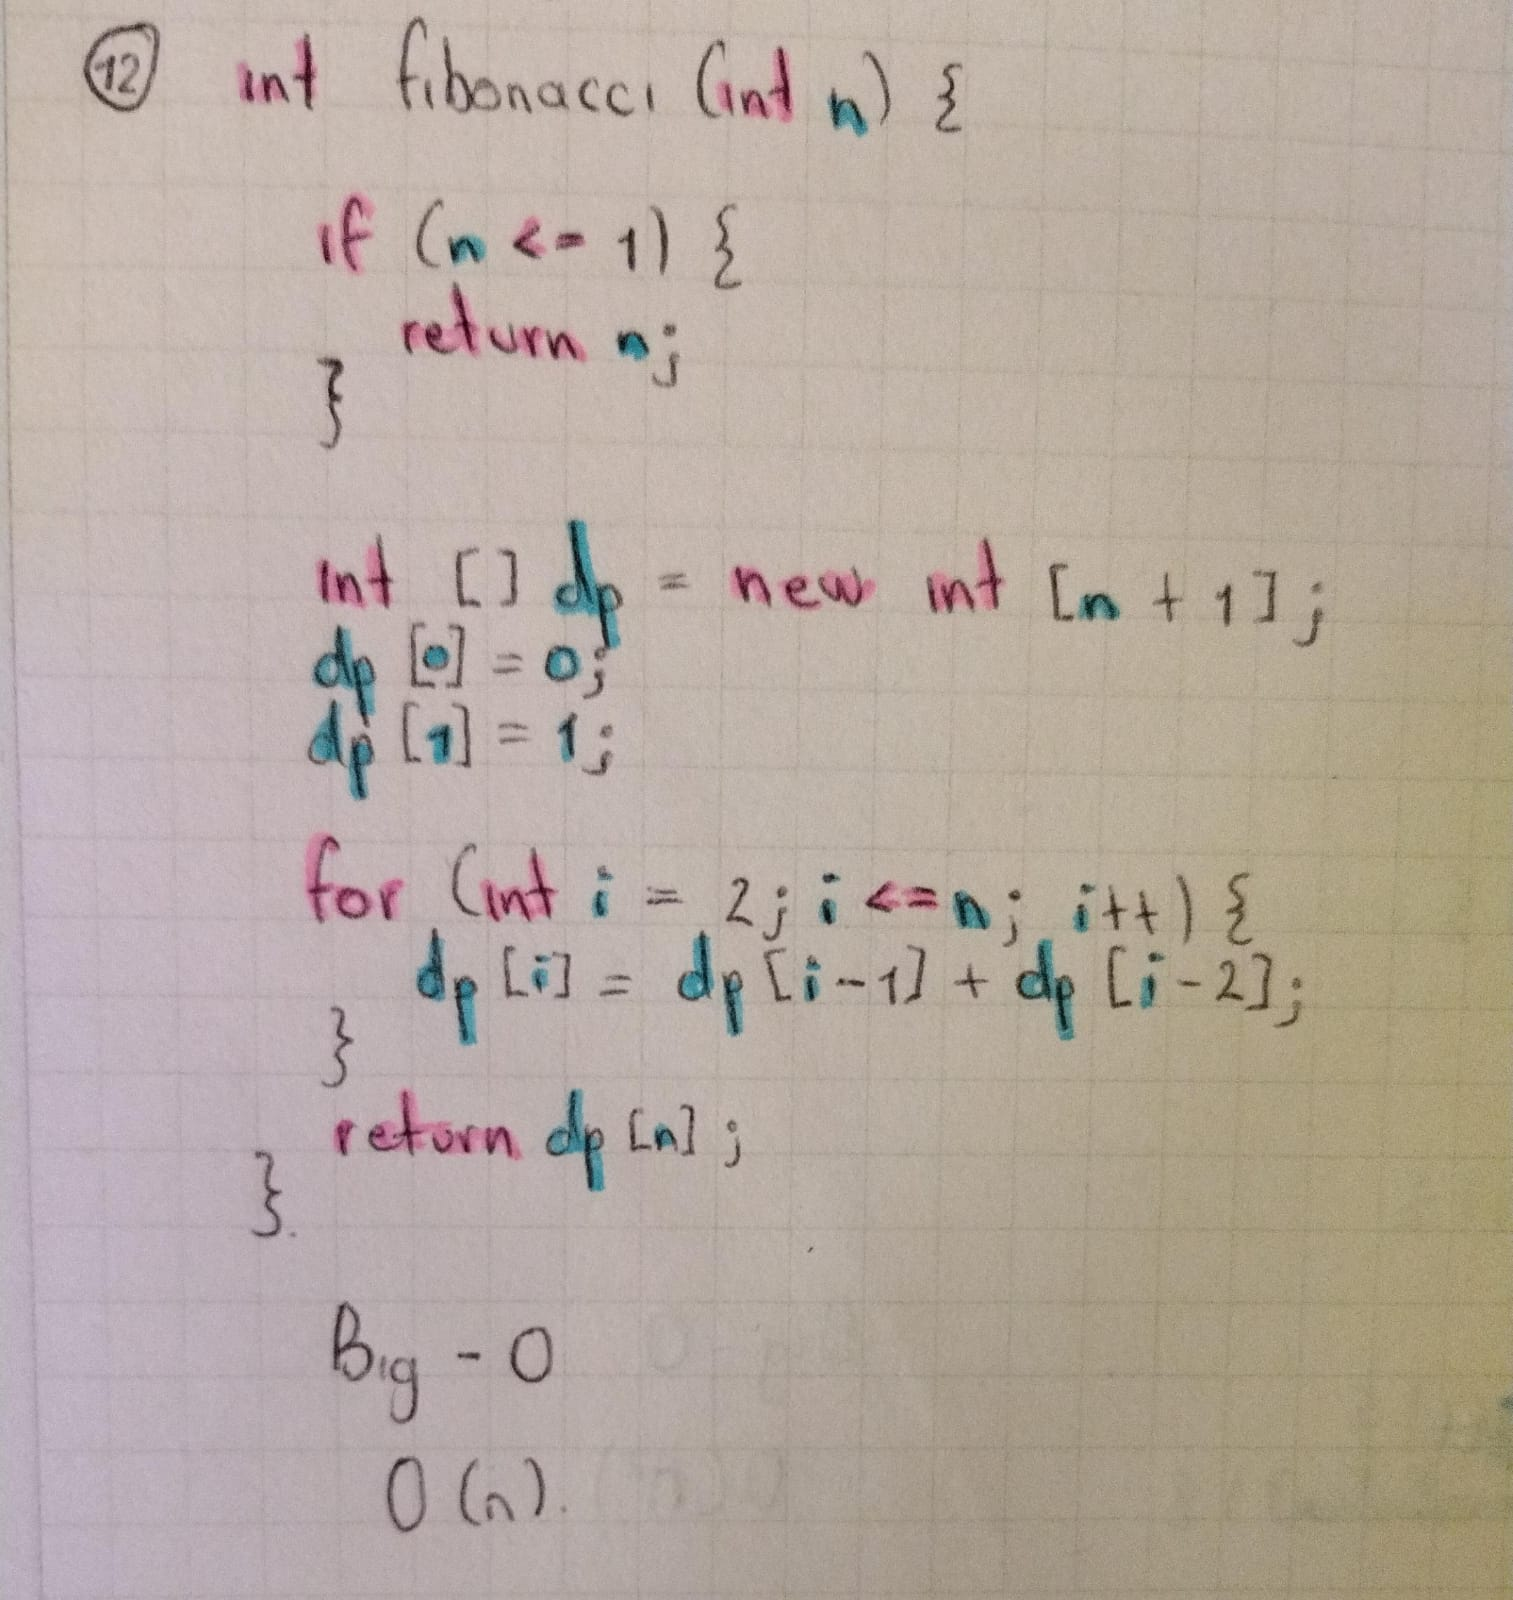
\includegraphics[width=1\linewidth]{imagenes/punto 12.jpeg}

\begin{itemize}
    \item La función fibonacci toma un solo argumento, "n", que representa el término de la secuencia de Fibonacci que se desea calcular.

     \item La primera condición $\texttt{if (n <= 1)}$ verifica si $n$ es menor o igual a $1$. Si es así, la función retorna $n$. Esto es una operación de tiempo constante: $O(1)$.

     \item Se crea un arreglo \texttt{dp} de tamaño "$\text n + 1$" para almacenar los valores de la secuencia de Fibonacci. Las operaciones de inicialización $\text dp[0] = 0$ y $\text dp[1] = 1$ son operaciones de tiempo constante: $O(1)$.

     \item En la siguiente línea se utiliza un bucle \texttt{for} para calcular los valores de la secuencia de Fibonacci desde el tercer término hasta el "n-ésimo" término. El bucle se ejecuta "$n-1$" veces en total. En cada iteración del bucle, se realiza una operación de asignación $\text dp[i] = dp[i - 1] + dp[i - 2]$. Esto también es una operación de tiempo constante: O(1).
     
\end{itemize}

La complejidad de tiempo de la función fibonacci es llevada bajo el bucle \texttt{for} que itera "$n-1$" veces. Por lo tanto, la complejidad de tiempo en el peor caso es $O(n)$.

\section{Código 13}
\begin{verbatim}
void linearSearch(int[] array, int target) {
for (int i = 0; i < array.length; i++) { // O(n)
        if (array[i] == target) { // O(1)
            // Encontrado
            return; // O(1)     
	   }
    }
    // No encontrado
}

\end{verbatim}

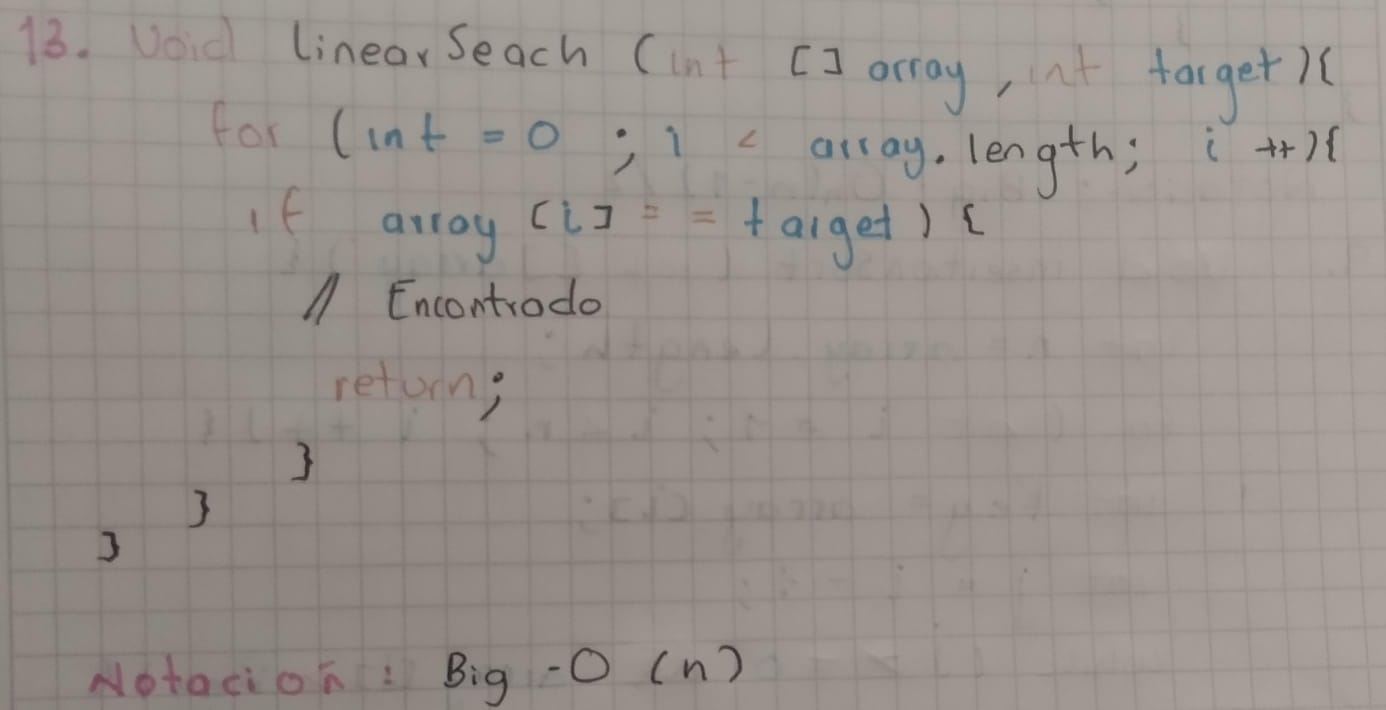
\includegraphics[width=1\linewidth]{imagenes/punto 13.jpeg}

\begin{itemize}

\item El bucle for itera a través de todo el arreglo con \texttt{array.length} elementos. Esto da como resultado una complejidad de $O(n)$, ya que la cantidad de iteraciónes depende directamente del tamaño del arreglo.

\item La comparación \texttt{if}  verifica si el elemento actual es igual al valor objetivo. Esta operación tiene una complejidad constante $O(1)$, ya que no depende del tamaño del arreglo

\item La línea \texttt{return;} detiene la función en caso de encontrar el elemento buscado. Esto también tiene una complejidad constante $O(1)$.

\item En el caso de no encontrar el elemento en todo el arreglo, simplemente se ejecuta la línea // No encontrado, la cual también tiene una complejidad constante $O(1)$.

\end{itemize}

Notacion Big – O:\\

La complejidad total del algoritmo es de $O(n)$ en el peor caso, ya que el bucle itera a través de todo el arreglo, y las operaciones dentro del bucle son de complejidad constante $O(1)$.

\section{Código 14}

\begin{verbatim}
    
int binarySearch(int[] sortedArray, int target) {
    int left = 0, right = sortedArray.length - 1;
    while (left <= right) {
        int mid = left + (right - left) / 2;
        if (sortedArray[mid] == target) {
            return mid; // Índice del elemento encontrado
        } else if (sortedArray[mid] < target) {
            left = mid + 1;
        } else {
            right = mid - 1;
        }
    }
    return -1; // Elemento no encontrado
}

\end{verbatim}

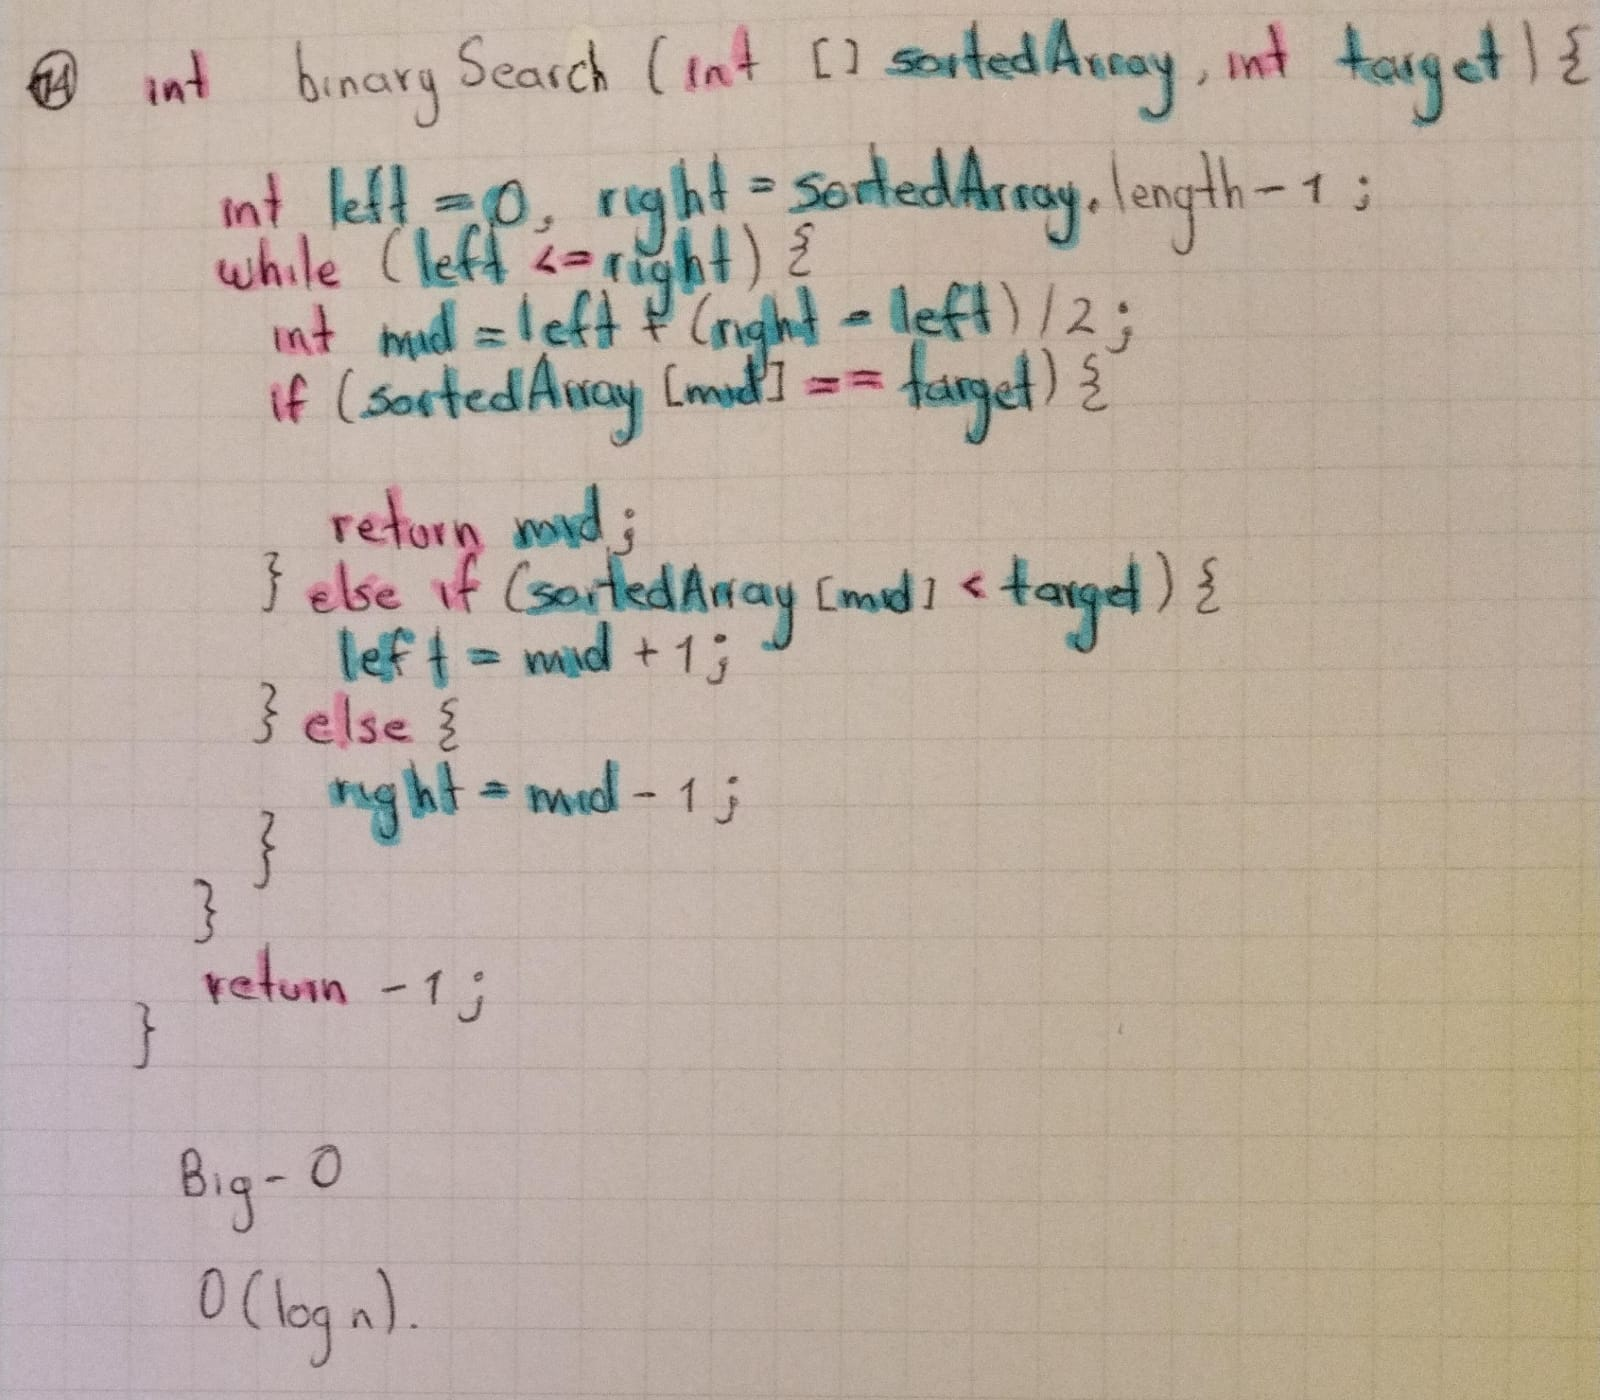
\includegraphics[width=1\linewidth]{imagenes/punto 14.jpeg}

\begin{itemize}

    \item Las líneas $\texttt{int left = 0, right = sortedArray.length - 1;}$ son asignaciones y tienen una complejidad de tiempo constante: $O(1)$.

    \item El bucle \texttt{while (left <= right)} se ejecuta mientras la condición \texttt{left <= right} sea verdadera. En cada iteración, el tamaño del rango en el que se está buscando se reduce a la mitad, ya que se actualizan los valores de \texttt{left o right} en función de si el elemento buscado es menor o mayor que el elemento en la posición \texttt{mid}.

    \item Dentro del bucle, se calcula el valor medio \texttt{mid} del rango de búsqueda actual. Esto se hace en tiempo constante: $O(1)$.

    \item Luego, se compara el en la posición mid con el elemento buscado target. Esta comparación es de tiempo constante: $O(1)$.

\end{itemize}

En resumen, la complejidad de tiempo de la búsqueda binaria es $O(log n)$ en el peor caso, donde $n$ es la longitud del arreglo ordenado\\



\section{Código 15}

\begin{verbatim}

int factorial(int n) {
    if (n == 0 || n == 1) {
        return 1;
    }
    return n * factorial(n - 1);
}

\end{verbatim}
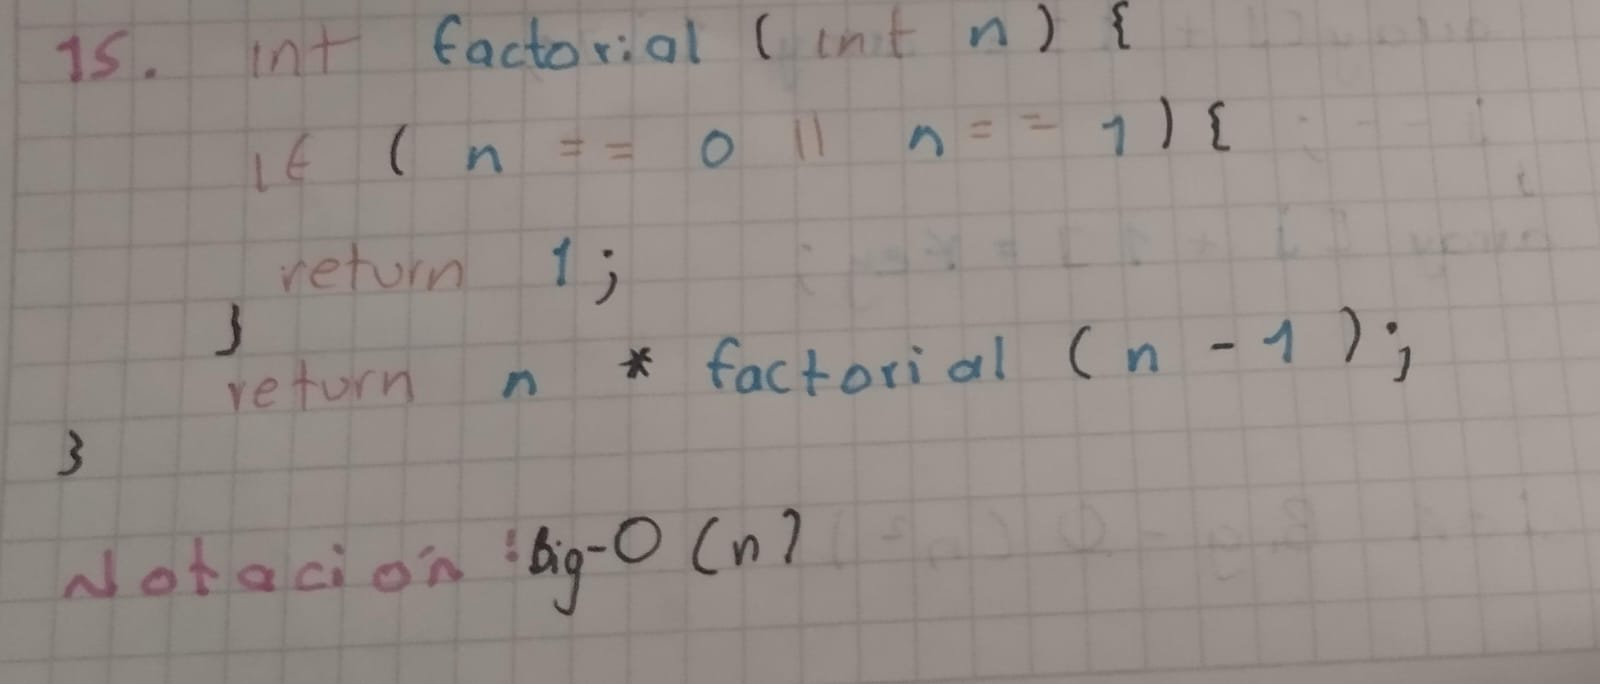
\includegraphics[width=1\linewidth]{imagenes/punto 15.jpeg}

\begin{itemize}

\item La línea del if  verifica si n es 0 o 1. Esta operación tiene una complejidad constante O(1), ya que no importa cuál sea el valor de n.

\item La línea \texttt{return 1;} devuelve $1$ cuando $n$ es $0$ o $1$. Esto también tiene una complejidad constante $O(1)$.

\item La línea return $\text n * factorial(n - 1);$ es donde se realiza la recursión. En cada llamada recursiva, se multiplica n por el resultado de la función \texttt{factorial($n - 1$)}. Dado que se realiza una llamada recursiva con un valor $n - 1$ y así sucesivamente hasta llegar a $\text n = 0 o n = 1.$ Esto nos dice que habrá $n$ llamadas recursivas en total, cada una realiza una multiplicación. Por lo tanto, la complejidad total de esta parte es $O(n)$.

\end{itemize}

Notacion Big – O:\\

La complejidad total de la función es $O(n)$, ya que el número de llamadas recursivas es directamente proporcional al valor de $n$, y cada llamada realiza una cantidad constante de trabajo (la multiplicación).

\end{document}

